\subsubsection{Sensitivity to dictionary size}
\label{subsubsection:rebuttal_dictionary_size}

We retrain the NLDisco models of \autoref{subsection:churchland_results} (macaque, $k=16$) and \autoref{subsection:aeon_results} (Aeon, $k=12$) with $D\in\{512,1024\}$, keeping two Matryoshka levels at $D/2$ and $D$ and every other setting, dataset, and training schedule unchanged, with three seeds per size. We compare them with the paper's $D=192$ models and the saved $D=128$ and $D=256$ runs (one seed each; for the macaque, five additional $D=192$ seeds and, for Aeon, two additional $D=192$ seeds serve as a seed-to-seed reference). The same analysis on a second Aeon session (session B, same animal, 18 hours of the preceding day) uses its own $D=192$ model as the reference.

\paragraph{Measures.}
A latent is \textit{dead} if it is never active ($z>0$) in any window. \textit{Training time} is the time for the paper's training schedule, estimated from interleaved short benchmarks on one GPU (minimum over repeats, because wall-clock times of full runs on shared GPUs vary several-fold with other jobs), together with the GPU time of a single optimization step. For each of the four feature descriptions of each dataset we apply the paper's selection rule at every size: among eligible latents (positive coverage $\geq0.05$, active in at least 20 trials or episodes), the one with the highest \metric{AUROC}; we report its \metric{AUROC} and \metric{Sel}. This rule recovers the paper's latents at their own size (Aeon) and the paper's best-\metric{AUROC} latents (macaque). To compare latents across models, we correlate their native activations over the same windows (all 130{,}507 macaque windows; all 3{,}238{,}600 Aeon windows). A latent of the paper's $D=192$ model \textit{reappears} if its maximum correlation with a live latent of the larger model is at least $0.5$. A live latent of the larger model is \textit{new} if no live latent of the paper's model correlates with it at $0.5$ or more, and a \textit{near-duplicate} if another latent of the same model correlates with it at $0.8$ or more. Both thresholds were fixed before the new runs were analyzed.

\paragraph{Results.}
Dead latents increase with $D$ (\autoref{figure:rebuttal_dictionary_size}a): from none at $D=192$ to $3$ at $D=512$ and $21$ at $D=1024$ (2\%) in the macaque model, and from none to $50$ (10\%) and $257$ (25\%) in the Aeon model; session B shows the same increase ($3$ at $D=192$, $52$, $248$). The GPU time of one optimization step grows with $D$, by $11\%$ (macaque) and $82\%$ (Aeon) at $D=1024$ relative to $D=192$; the end-to-end schedule time grows by $53\%$ for Aeon ($93$ to $143$ s) and is unchanged for the macaque ($68$ s at both sizes), whose training loop is dominated by data loading (\autoref{figure:rebuttal_dictionary_size}b).

The paper's features persist at every size. The best-\metric{AUROC} latent for each description stays between $0.77$ and $0.99$ (\autoref{figure:rebuttal_dictionary_size}c,d), for example \textit{early leftward movement} $0.98$ at $D=192$ and $0.98$ at $D=1024$ and \textit{wheel activity} $0.92$ and $0.90$. Between $88\%$ and $92\%$ of the paper model's latents reappear at $D\geq256$ in the macaque and Aeon models and in session B, against $86\%$ (macaque) and $88\%$ (Aeon) between independently trained $D=192$ models (\autoref{figure:rebuttal_dictionary_size}e). The additional latents are mostly new: $69\%$ of the live latents at $D=1024$ in the macaque model ($691$ latents) and $57\%$ in the Aeon model ($439$ latents) have no counterpart in the paper's model, compared with $14\%$ and $12\%$ between $D=192$ seeds. In the macaque model, near-duplicates are essentially absent at every size (at most two latents). In the Aeon models, $34\%$ of the live latents of the paper's model are near-duplicates, and the share does not grow with size ($26\%$ at $D=1024$).

\begin{figure}[!htbp]
    \centering
    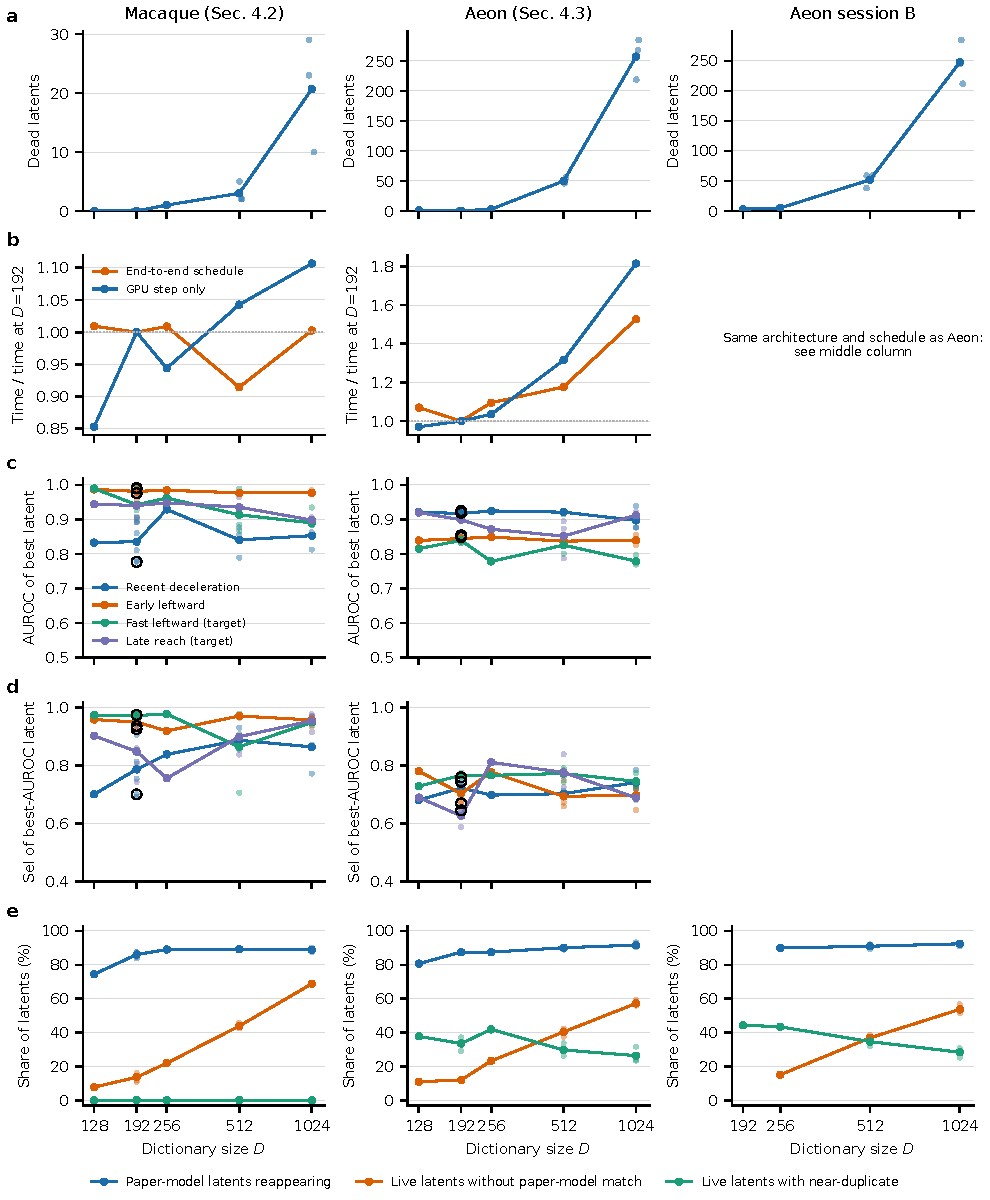
\includegraphics[width=\linewidth]{figures/rebuttal/change08_dictsize/dictionary_size.pdf}
    \caption{\textbf{Dictionary-size sensitivity.} Columns: macaque model (Section~\ref{subsection:churchland_results}; $k=16$), Aeon model (Section~\ref{subsection:aeon_results}; $k=12$), and Aeon session B ($k=12$). Small dots are individual runs; lines connect means (three seeds at $D=512,1024$; macaque $D=192$: six seeds; Aeon $D=192$: three seeds; one seed otherwise). Open circles mark the paper's $D=192$ model. (\textbf{a}) Dead latents. (\textbf{b}) Training time relative to $D=192$: paper schedule (orange) and one optimization step on the GPU (blue). (\textbf{c,d}) \metric{AUROC} and \metric{Sel} of the best-\metric{AUROC} eligible latent for each of the paper's four feature descriptions (legend in c; Aeon: wheel activity, smaller area near the patch, fast centroid speed, fast outward movement). (\textbf{e}) Share of the paper's $D=192$ latents that reappear in the larger model (activation correlation $\geq0.5$), share of the larger model's live latents without such a counterpart, and share of live latents with a near-duplicate (correlation $\geq0.8$) in the same model; $D=192$ points compare independent seeds.}
    \label{figure:rebuttal_dictionary_size}
\end{figure}
